\documentclass[12,french]{report}
\usepackage{geometry}
\geometry{vmargin=3cm, hmargin=3cm}
\usepackage[T1]{fontenc}
\usepackage[utf8]{inputenc}
\usepackage[french]{babel}
\usepackage{graphicx}
\usepackage{amsmath}
\usepackage{amssymb}
\usepackage{sectsty}
\usepackage{authblk}
\usepackage{algpseudocode}
\usepackage{algorithm}
\usepackage{xspace}
\usepackage{mathtools}
\usepackage{mathrsfs}
\usepackage{enumitem}
\usepackage{titlesec}
\usepackage{hyperref}
\usepackage{xcolor}
\usepackage[justification=centering]{caption}
\usepackage{float}
\usepackage{tabto}

\usepackage{listings}
\usepackage{cleveref}

\renewcommand{\lstlistingname}{Code}
%\renewcommand{\figurename}{Fig.}

\lstdefinestyle{chstyle}{%
backgroundcolor=\color{gray!12},
basicstyle=\ttfamily\small,
showstringspaces=false,
numbers=left}

%\AddThinSpaceBeforeFootnotes
%\FrenchFootnotes

\titleformat{\chapter}[hang]{\bf\Huge}{\thechapter.}{2pc}{}
\titlespacing*{\chapter}{10pt}{0pt}{40pt}[0pt]
\newcommand{\HRule}{\rule{\linewidth}{0.5mm}}

\providecommand{\keywords}[1]{\textbf{\textit{Keywords:}} #1}
\bibliographystyle{apalike}

\usepackage{hyperref}

\begin{document}
\hypersetup{pdfborder=0 0 0}

\begin{titlepage}

\begin{center}
	\vspace*{\stretch{1}}
	\textsc{{\LARGE Institut national des sciences appliquées de Rouen} \\ 			\vspace{6mm} {\Large INSA de Rouen}} \\
	\vspace{5mm}
	
\includegraphics[width=0.4\textwidth]{./Images/insa}\\[1.0 cm]

	\textsc{\Large Projet INFO GM3 - Vague 1 - Sujet 4}\\[0.6cm]

	% Title
	\HRule \\[0.5cm]
	{ \Huge \bfseries Réalisation d'une salle d'ordinateur Java}\\[0.2cm]
	\HRule \\[0.75cm]

	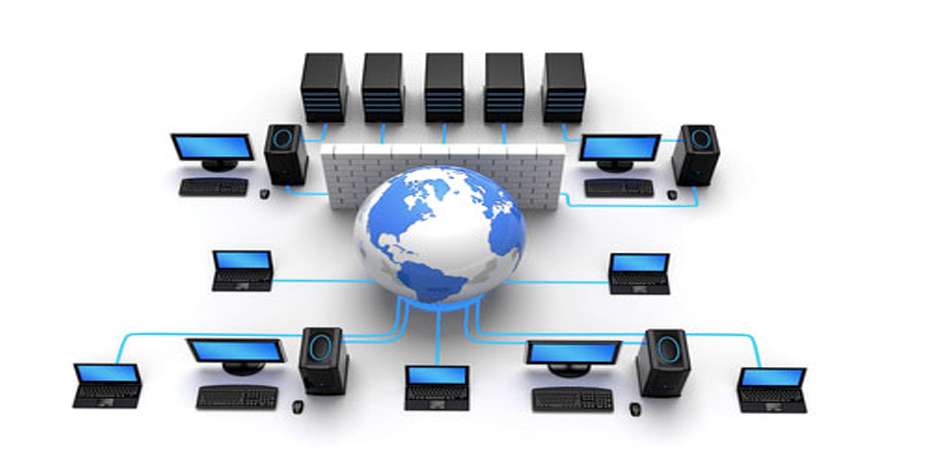
\includegraphics[width=0.7\textwidth]{./Images/pagedegarde}\\[0.9 cm]

	% Author and supervisor
	\begin{minipage}{0.4\textwidth}
		\begin{flushleft} \large
			\emph{Auteurs:}\\
			Thibaut \textsc{André-Gallis} \\
			{\small\href{mailto:thibaut.andregallis@insa-rouen.fr}{thibaut.andregallis@insa-rouen.fr}} \\
			Kévin \textsc{Gatel} \\
			{\small\href{mailto:kevin.gatel@insa-rouen.fr}{kevin.gatel@insa-				rouen.fr}}
		\end{flushleft}
	\end{minipage}
	\begin{minipage}{0.4\textwidth}
		\begin{flushright} \large
			\emph{Enseignants:} \\
			Habib \textsc{Abdulrab} \\
			{\small\href{mailto:habib.abdulrab@insa-rouen.fr}{habib.abdulrab@insa-rouen.fr}}
		\end{flushright}
	\end{minipage}
	\vspace*{\stretch{1}}

	\vfill
	{\large 19 Février 2021}
\end{center}
\end{titlepage}

\tableofcontents

%\listoffigures

\renewcommand{\chaptername}{}
\chapter*{Introduction}

Le mini-projet que nous avons choisi est la réalisation d'une salle d'ordinateur en Java.\\

Nous allons donc programmer une salle d'ordinateur en Java. C'est à dire que nous allons créer un programme qui simulera la gestion d'une salle d'ordinateur comme on pourrait le rencontrer à l'INSA par exemple. Cette salle sera composée d'ordinateurs évidemment mais pas seulement. Nous allons y ajouter de nombreux appareils électroniques comme des routeurs, imprimantes... Afin de se rapprocher au plus possible de la réalité. Les appareils auront la possibilité d'interagir entre eux pour certaines actions. \\

Le but de ce projet est d'utiliser habilement les concepts de la programmation objet, c'est-à-dire savoir écrire les différents diagrammes, maîtriser l'héritage entre les classes, le polymorphisme, la gestion des interfaces ou des classes arbitraires, etc...\\

Pour bien répondre au problème, nous allons d'abord nous concentrer sur le \textbf{diagramme de classe} (UML) afin de comprendre l'organisation du code que nous allons implémenter.\\

Ensuite, nous allons présenter et décrire le rôle de \textbf{chacune des classes} qui ont été nécessaires à la réalisation du projet.\\

Enfin, nous verrons \textbf{les différents problèmes} que nous avons pu rencontrer lors de la programmation du jeu.


\chapter{Le diagramme}

\section{UML}

\begin{figure}[H]
	\center
	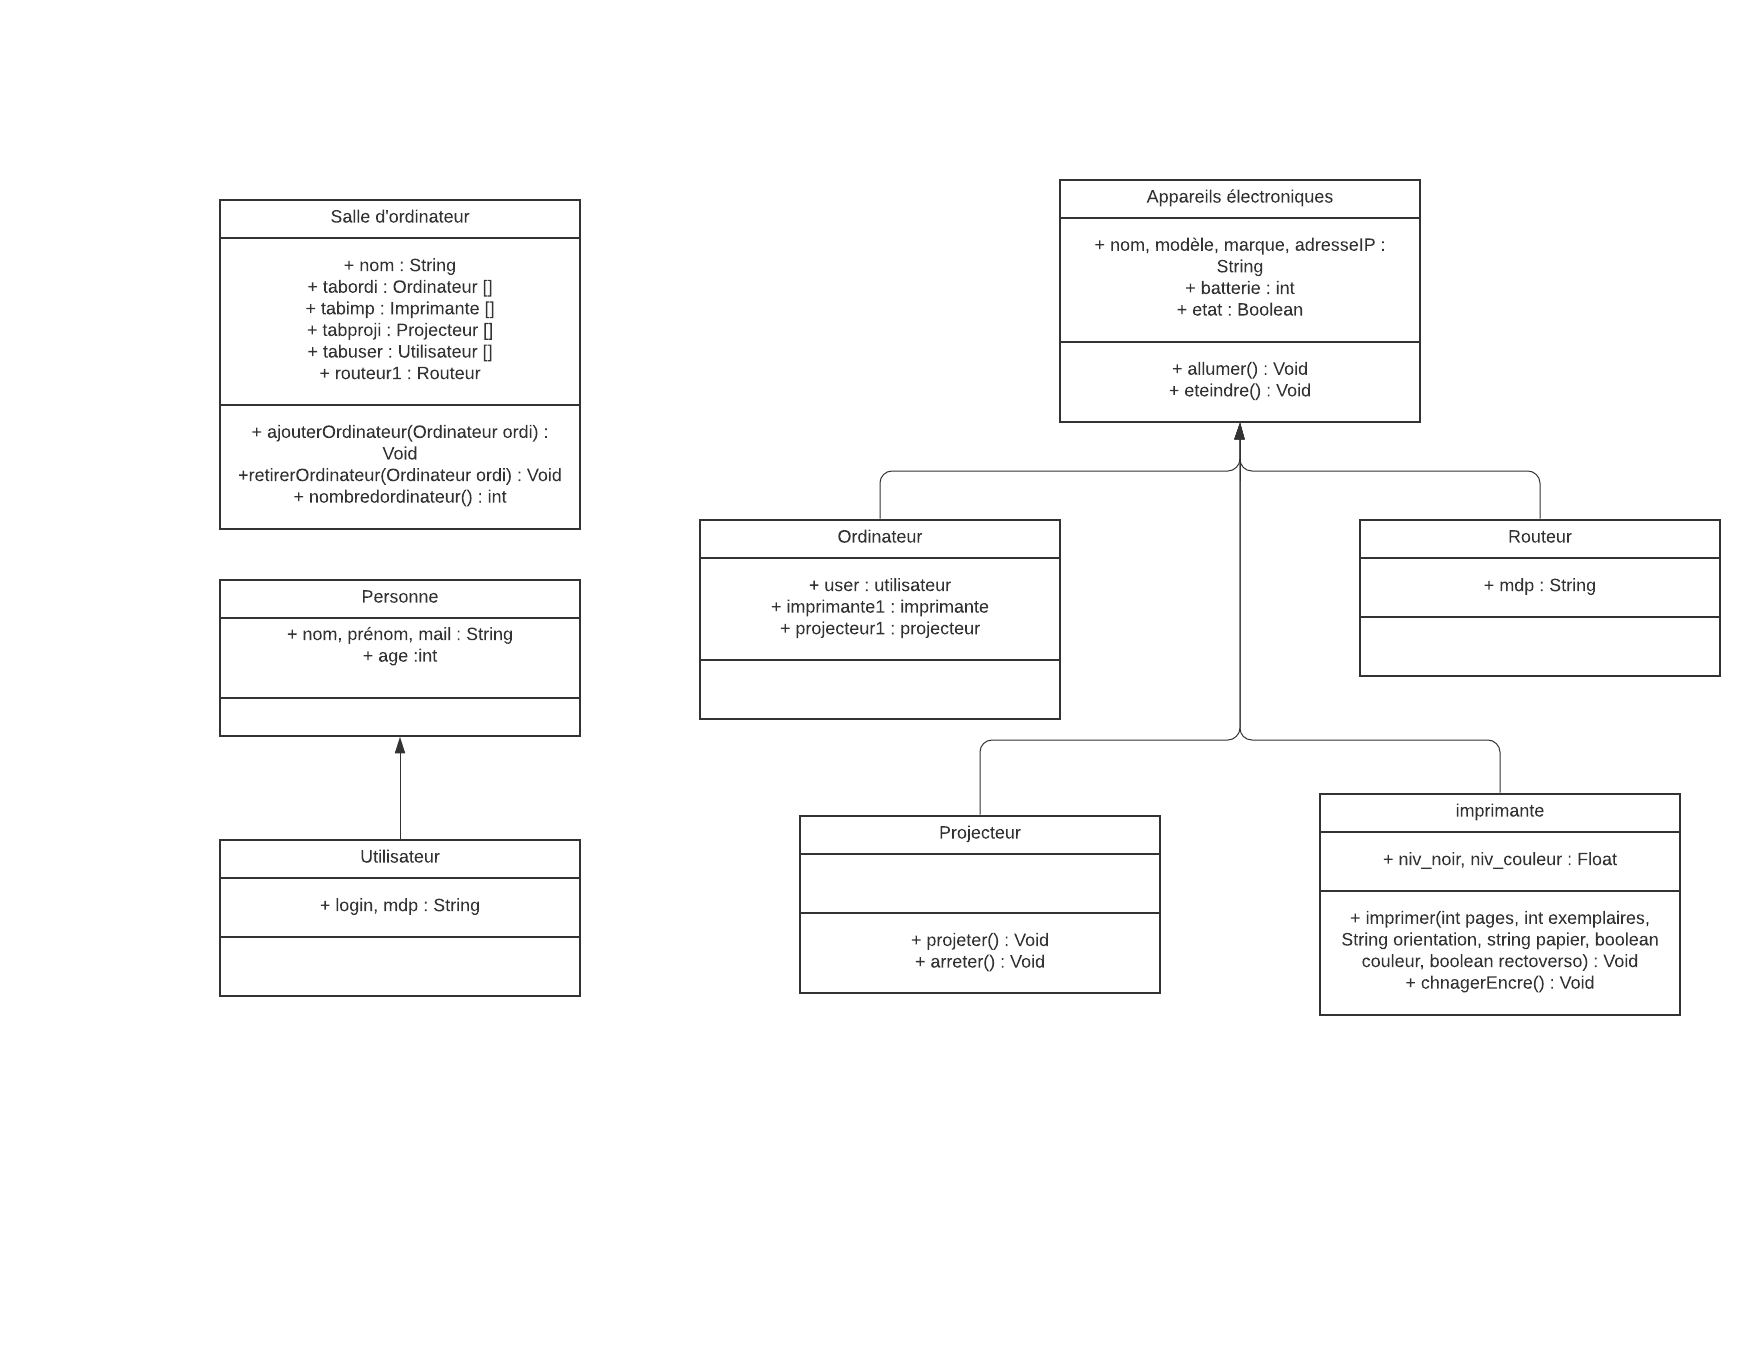
\includegraphics[width=1\textwidth]{./Images/UML}
	\caption{Diagramme de classe pour la salle d'ordinateur}
\end{figure}\vspace{0.2cm}

Nous avons donc penser le programme en une classe salle d'ordinateur qui va donc correspondre à celle du sujet. Cette classe centrale va servir de lien entre tout les appareils électroniques de la salle. En effet elle va contenir dans des tableaux plusieurs éléments de chaque type et grâce à un menu, elle va permettre d'accéder à  tous les éléments de la salle et d'effectuer différentes actions sur chacun.\\

On a également pensé à une autre classe commune à de nombreux éléments, la classe appareil électronique. Cette classe regroupe tous les types d'appareils possible que l'on peut rencontrer dans une salle d'ordinateur et chacun des différents types d'appareils vont hériter de cette classe commune.\\

Un autre élément important, la gestion des personnes et utilisateurs de la salle. Les utilisateurs hériteront de la classe Personne et ils permettront de se connecter aux ordinateurs. Nous avons également pensé à différencier les différents profils d'utilisateurs tel que les élèves et les professeurs qui n'auront donc pas les même droits d'action sur certains appareils.


\chapter{Les classes}

\section{Salle d'ordinateur}

La classe \textit{Salle d'ordinateur} est la classe principale du programme. Elle va donc posséder un nom un tableau d'ordinateur, un tableau d'imprimante, un tableau de projecteur, un tableau d'utilisateur et un routeur. Ce sont tous les éléments de la salle. Elle va posséder des méthodes plutôt simple tel qu'un menu afin d'accéder à tous les éléments de la salle, Une méthode d'ajout et de retrait pour chaque appareil électronique différents. Mais également une méthode \textit{toString} redéfini afin de pouvoir afficher l'ensemble de la salle.

\section{Personne}

La classe \textit{Personne} ne possède aucune méthode. Elle a été créée dans le seul but d'être hérité par la classe Utilisateur et elle possède des informations inhérentes à chaque personne tel que le nom, le prénom... 

\section{Utilisateur}

La classe \textit{Utilisateur} possède deux variables d'instance login et mdp qui vont servir à  se connecter à un ordinateur et donc débloquer certaines fonctions uniquement disponible si un utilisateur est connecté sur l'ordinateur.

\section{Eleve}

La classe \textit{Eleve} ne possède rien hormis le fait qu'elle existe. Elle sert juste à différencier les élèves et les professeurs ce qui a un impact sur certaines fonctionnalités.

\section{Professeur}

De même la classe \textit{Professeur} ne possède rien mais elle se différencie avec la classe élève juste en existant.

\section{Appareils électroniques}

La classe \textit{Appareils électroniques} regroupe les caractéristiques communes à tous les appareils comme le modèle, la marque...\\
Elle possède deux méthodes \textit{allumer()} et \textit{eteindre()} qui servent à allumer et éteindre un appareil en agissant sur leur variable etat qui est un booléen.

\section{Ordinateur}

La classe \textit{Ordinateur} correspond à un ordinateur. Depuis celui-ci on peut se relier à une imprimante, un routeur ou un projecteur. On peut aussi se connecter avec un utilisateur et imprimer un document ou le projeter. On peut également grâce au routeur se connecter à internet.

\section{Routeur}

La classe \textit{Routeur} possède uniquement un mot de passe qui permet de se connecter à un internet avec un ordinateur

\section{Projecteur}

La classe \textit{Projecteur} permet de projeter et d'arrêter la projection d'un document à partir d'un ordinateur.

\section{imprimante}

La classe \textit{Imprimante} possède son niv d'encre de couleur et noir, et elle permet une fois relié à un ordinateur d'imprimer un document. On peut aussi recharger son niveau d'encre.

\section{Main}

La classe \textit{Main} et le programme principal de la salle. Elle consiste en une salle d'ordinateur et un vaste menu permettant d'accéder à tous les éléments de la salle et d'effectuer toutes les actions que l'on souhaite.

\chapter{Problèmes rencontrés}

\section{Modélisation}

Tout d'abord nous avons eu des difficultés à imaginer le programme. En effet comme c'était notre tout premier programme informatique en programmation par objet, le concept était tout nouveau pour nous. Nous avons d'abord pensé à tout faire d'un coup comme nous avions l'habitude de faire mais nous n'aurions eu aucun intérêt à le faire en Java. Notre première difficulté a donc été de penser par objet. Une fois que nous avions fait un brouillon des différentes classes que nous imaginions nous les avons remanié afin d'y intégrer la notion d'héritage car nous nous sommes rendus compte que certaines classes différents avaient des paramètres en commun qui pouvait se rassembler en une classe mère. Il a ensuite fallu réaliser notre premier diagramme de classe selon le modèle UML et même si cela n'a pris longtemps à comprendre comment cela fonctionnait c'était nouveau pour nous.

\section{Le programme principal}

Une autre difficulté plus surprenante à laquelle nous avons du faire face et la réalisation du programme principal, c'est à  dire la classe \textit{Main}. En effet paradoxalement une fois que nous avions pensé le programme par objet et implémenter les différentes classes et leur classe test respectives. Nous nous sommes rendus compte que nous n'avions pas de classe main nous permettant de faire tourner notre programme et ses classes. Nous avons donc réfléchi à la façon de faire et nous sommes partis sur une sorte de vaste menu permettant d'afficher et d'explorer la salle puis d'agir sur chacun des éléments de la salle. Ce menu se devait d'être récursif et qu'il ne s'arrête que lorsque l'utilisateur le souhaite. Nous avons du utiliser des variables locales choix pour définir la volonté de l'utilisateur et nous avons dû les réinitialiser à leur valeur dd'origine à chaque choix afin que le programme ne s'arrête jamais. Ce point en particulier nous a pris du temps à résoudre car notre menu finissait par s'arrêter et nous ne comprenions pas pourquoi.
 
\chapter*{Conclusion}
\addcontentsline{toc}{chapter}{Conclusion}

Pour commencer ce projet nous a été très enrichissant d'un point de vue programmation évidemment. En effet il a constiuté notre tout premier programme dans le langage Java et surtout notre premier programme en programmation par objet.\\
Cela nous a permis de découvrir la programmation par objet et ses intérêts en utilisant uniquement des éléments de base et nos connaissances en programmation classique. Le projet étant réalisé au tout début du semestre, il nous a permis d'appréhender le cous avec plus de facilité et même de prendre de l'avance par nous même sur certaines notions du cours.\\
Cela a été également l'occasion pour nous de découvrir le diagramme de classe et le langage UML ainsi que son importance pour structurer avant de coder. De plus les diagrammes sont très important pour faciliter la compréhension du programme à une personne extérieur qui pourrait être amené à travailler sur le programme.\\

Enfin il fût intéressant de pouvoir construire ce programme avec à la base deux façons différentes de voir le programme puis d'arriver à une solution composé des deux qui regroupe les avantages des deux. La complémentarité de nos deux points de vue a permis de réaliser quelque chose qu'il n'aurait pas été possible de faire seul.\\

Pour conclure, nous avons vraiment apprécié prendre part à ce projet et cela nous a permis de nous initier au langage Java et d'acquérir des bases dans ce langage qui nous seront utile pour la suite.

\end{document}
